\documentclass[10pt, titlepage, a4paper]{article}

\usepackage{kcp}

\def\npredmet{Zaključna naloga MAF2}

\bibliography{refs.bib} %insert .bib file

% when compiling run
% pdflatex <main>.tex
% biber <main>[.bcf]
% pdflatex <main>.tex
% pdflatex <main>.tex

\title{
\includegraphics[width=0.25\textwidth]{./figures/fmf_logo}\\
  {\small Oddelek za fiziko} \\
  Naloga 20: Vrv \\
  {\small Zaključna naloga pri predmetu Matematična fizika 2} \vspace{2cm}
\begin{center}\begin{minipage}[c]{0.9\textwidth}\centering \footnotesize Obravnavaj nihanje dolge težke vrvi obešene na strop [\textit{verjetno bo potrebna numerika}].\end{minipage}\end{center}}

\author{Kristofer Čepon Povšič, 28211104 \\
\small{Profesor: Marko Žnidarič}}

\date{Julij, 2026}


% page header

\pagestyle{fancyplain}
\ifx\ncoursehead\undefined
  \def\ncoursehead{\npredmet}
\fi

\lhead{\emph{\nouppercase{\leftmark}}}
\rhead{
  \ifnum\thepage=1
  \else
    \ncoursehead
  \fi
}

\setlength\parindent{0pt}

\begin{document}
\pagenumbering{gobble} % remove counter from first page

\maketitle

\pagenumbering{arabic}
\tableofcontents

\newpage
\section{Teoretični model}
\subsection{Izpeljava valovne enačbe}

V sklopu predavanj predmeta Matematična fizika 2 smo izpeljali valovno enačbo za struno. Izpeljavo bom tukaj ponovno povzel zaradi celovitosti naloge.

Vrv dolžine \( L \) s konstantno dolžinsko gostoto \( \mu \) visi s stropa, kakor prikazuje slika \ref{fig:koordinate}. Odmiki vrvi naj bodo majhni glede na koordinatno os \( x \) in pravokotni nanjo (naša slika je torej močno pretirana).

\begin{figure}[htbp]
\centerline{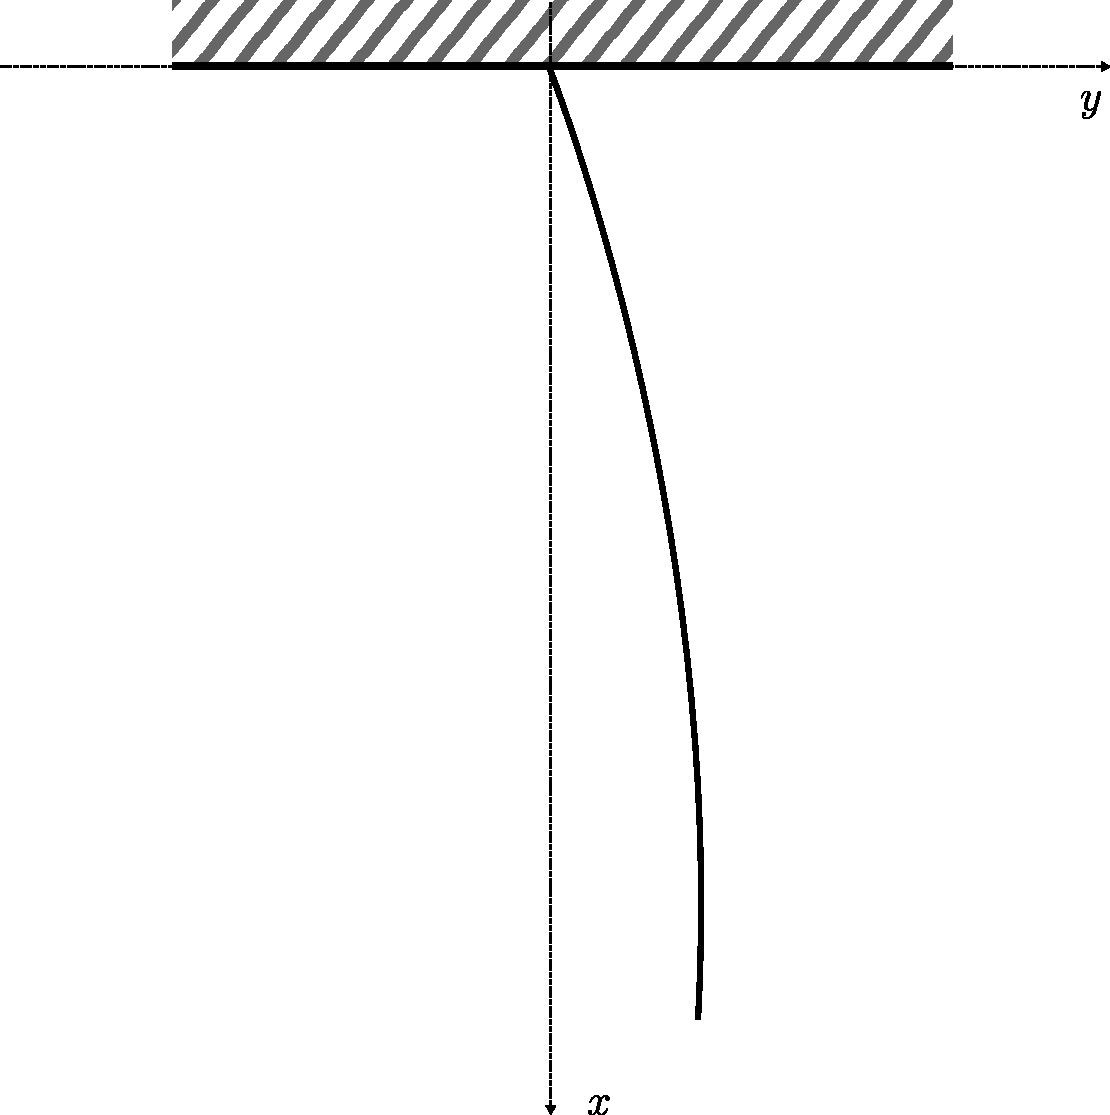
\includegraphics[width=0.45\textwidth]{figures/koordinate.pdf}}
\caption{\small Skica našega problema - težka vrv, ki visi s stropa.\label{fig:koordinate}}
\end{figure}

Opazujemo košček vrvi dolžine \( \mathrm{d} s \) in sile, ki delujejo na njega, kot je prikazano na sliki \ref{fig:koscekVrvi}.

\begin{figure}[htbp]
\centerline{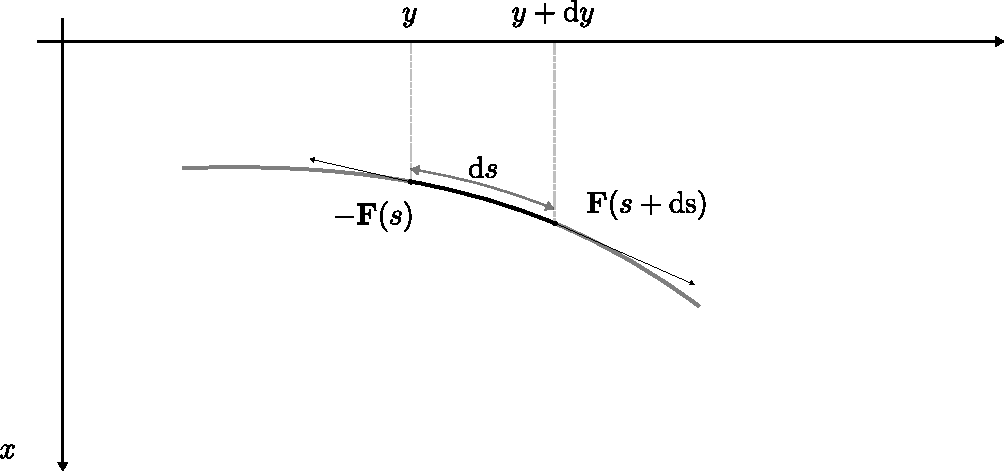
\includegraphics[width=0.60\textwidth]{figures/delcekvrvi.pdf}}
\caption{\small Košček vrvi \( \mathrm{d} s \) in sile, ki delujejo na njega. \label{fig:koscekVrvi}}
\end{figure}

Edina zunanja sila, ki deluje na vrv, je sila teže \( F_x = \mu (L - x) g \). Preko definicije kosinusa zapišemo

\[ F_y = F \frac{\mathrm{d} y}{\mathrm{d} s}. 
\]
Ker so odmiki v smeri \( x \) majhni (\( \mathrm{d} x \ll \mathrm{d} y \)), lahko dolžino loka \( \mathrm{d} s \) nadomestimo s projekcijo \( \mathrm{d} y \). Enako lahko storimo tudi z razliko nateznih sil

\[ \mathbf{F}(s + \mathrm{d}s) - \mathbf{F}(s) = \frac{\partial }{\partial s} F_x = \frac{\partial }{\partial s} \left( F \frac{\mathrm{d} x}{\mathrm{d} s} \right).
\]
Razlika nateznih sil po drugem Newtonovem zakonu struno pospešuje, zato zapišemo

\[ \mu \frac{\partial ^2 y}{\partial t ^2} = \frac{\partial }{\partial s} \left( F \frac{\mathrm{d} x}{\mathrm{d} s} \right)  
\]


\subsection{Definicija problema}
\subsection{Splošna rešitev}
\subsection{Začetni pogoji}

\section{Numerični izračuni}

Občasno, ko vrv prosto visi z vrha plezalne smeri, njen prost konec udarim z roko in opazujem dogajanje. Lokaliziran udarec je \( \delta \) funkcija, ki pa jo aproksimiramo s Heavisideovo funkcijo na zadnji \( 5\% \) vrvi

\[ f(x) = v_0 \theta(x - 0.95 * L) 
\]

Za numerične izračune si zamislimo vrv z dolžino \( L = 1 \mathrm{m} \), začetno hitrost \( v_0 = 1 \frac{\mathrm{m}}{\mathrm{s}} \) in gravitacijski pospešek je \( g = 9.81 \frac{\mathrm{m}}{\mathrm{s} ^2} \).

\section{Zaključek}

Tekom naloge smo definirali matematičen problem, ki ga predstavlja s stropa pritrjena težka vrv. Potrdili smo, da z uporabljenimi metodami Fourier-Besslova vrsta konvergira v \( L^2 \) prostoru. Izbrali smo si optimalno število členov, ki nima prevelike časovne zahtevnosti, s katerimi smo si potem ogledali časovni razvoj vrvi. Prav tako smo potrdili konvergenco kumulativne vsote koeficientov.

Možne izboljšave so nadomestilo trapezne metodo z npr. Newtonovo metodo pri numerični integraciji. Zanimivo bi si bilo ogledati časovni razvoj vrvi za različne druge začetne pogoje. 
\printbibliography[heading=bibintoc]
\end{document}
